% Created 2026-03-02 Mon 20:30
% Intended LaTeX compiler: pdflatex
\documentclass[hidelinks, 12pt]{article}

\usepackage[utf8]{inputenc}
\usepackage[T1]{fontenc}
\usepackage{graphicx}
\usepackage{longtable}
\usepackage{wrapfig}
\usepackage{rotating}
\usepackage[normalem]{ulem}
\usepackage{amsmath}
\usepackage{amssymb}
\usepackage{capt-of}
\usepackage{hyperref}
\makeatletter \@ifpackageloaded{geometry}{\geometry{margin=2cm}}{\usepackage[margin=2cm]{geometry}} \makeatother
\usepackage{siunitx}
\usepackage{amsmath}
\usepackage{amssymb}
\usepackage{mathtools}
\usepackage{circuitikz}
\usepackage{float}
\usepackage{karnaugh-map}
\usepackage{libertine}
\usepackage[libertine,cmintegrals,cmbraces,vvarbb]{newtxmath}
\usepackage[scaled=0.95]{zi4}
\usepackage{fancyhdr}
\pagestyle{fancyplain}
\lhead{Bach \textsc{Wongwandanee}}
\rhead{ECE 403}
\chead{Assignment 7}
\author{Waridh (Bach) Wongwandanee}
\date{\today}
\title{ECE 403 Assignment 7}
\hypersetup{
 pdfauthor={Waridh (Bach) Wongwandanee},
 pdftitle={},
 pdfkeywords={},
 pdfsubject={},
 pdfcreator={},
 pdflang={English}}
\usepackage{biblatex}

\begin{document}

\section*{Question 1}
\label{sec:orgd666d93}
Find the fastest safe clock frequency for a 3-cycle
pipeline that feeds back on itself. Solve using D-FFs
for synchronization. Verify that hold time is met.
\begin{itemize}
\item \(T_{skew} = \qty{0}{\pico\s}\)
\item 7 stages of combinational logic, each with \(T_{cd-group} = \qty{100}{\pico\s}\) and, used in the provided sequence, \(T_{pd}=\left\{ {500, 600, 300, 400, 500, 200, 110} \right\} \unit{\pico \s}\).
Synchronize the \qty{110}{\pico\s} stage output to the clock.
\item latches and D-FFs : \(T_{setup}=\qty{40}{\pico\s}, T_{hold}=\qty{30}{\pico\s}, T_{pcq}=\qty{45}{\pico\s}, T_{ccq}=\qty{30}{\pico\s}, T_{pdq}=\qty{50}{\pico\s}, T_{cdq}=\qty{35}{\pico\s}\)
\end{itemize}

We are going to start off with our assumptions.
We assume here that the combinational component must be executed in order, and the order is given by listing in the question.
This means that you could only group stages adjacent to each other.
Additionally, there shall be 3 stages of combinational logic.
With these assumptions, we can now start to build our pipeline.

In our vision, the new pipeline shall have the following grouping of combinational circuits.

\begin{verbatim}
{500 + 600, 300 + 400, 500 + 200 + 100}
\end{verbatim}

Where the first and second group has two stages, and the third group has 3 stages.
The system is available in figure \ref{fig-schematic}.

\begin{figure}[htbp]
\centering
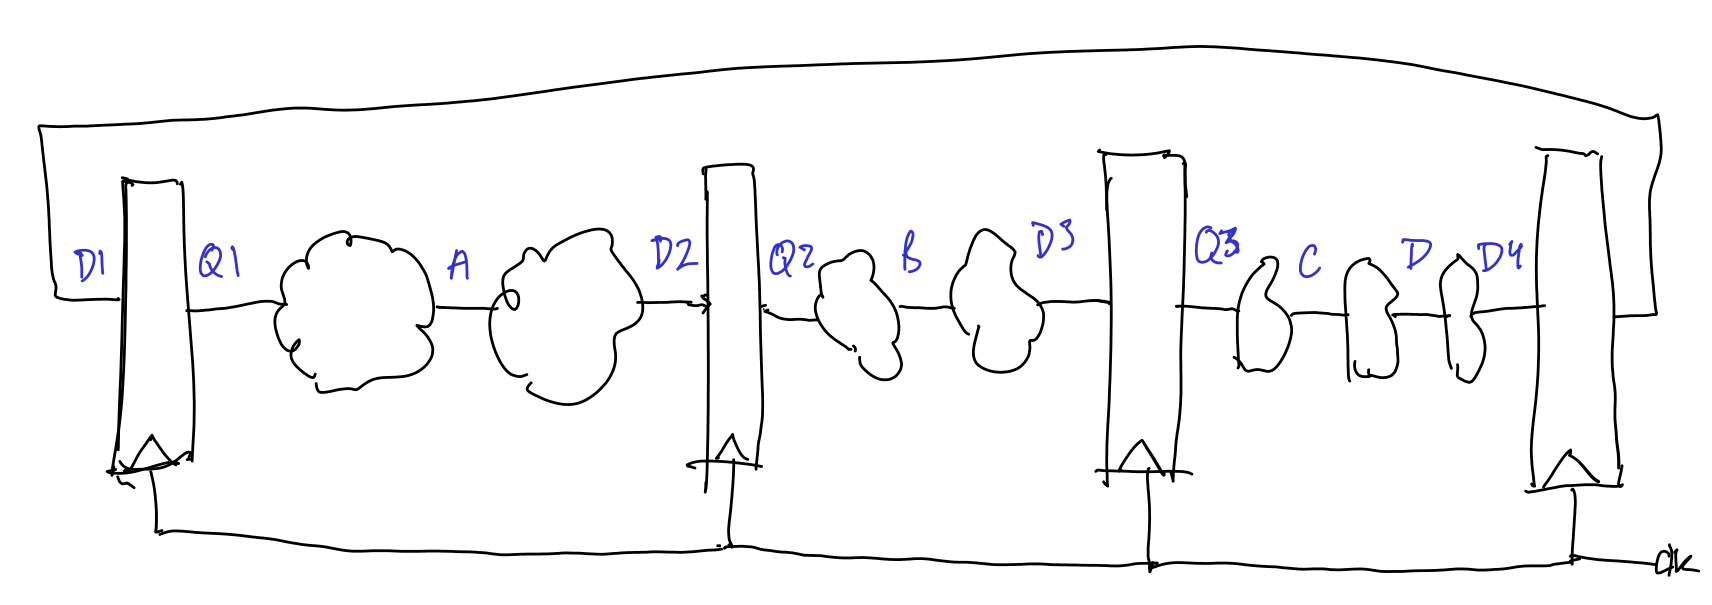
\includegraphics[width=0.7\linewidth]{images/schematic.png}
\caption{\label{fig-schematic}The block diagram for the proposed system.}
\end{figure}

\begin{figure}[htbp]
\centering
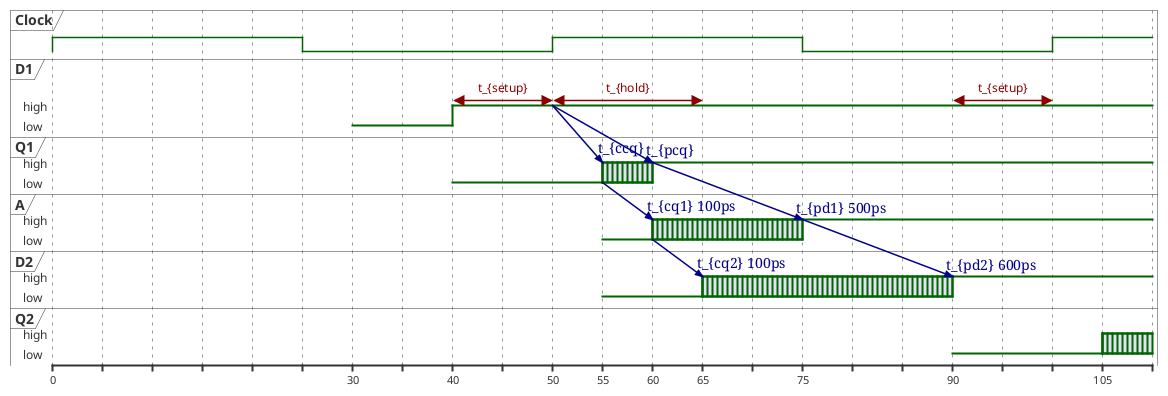
\includegraphics[width=0.7\linewidth]{./images/q1-timing.png}
\caption{\label{lst-q1-timing}Timing diagram used to understand how the configuration of the system affects the timing parameters.}
\end{figure}
\section*{Question 2}
\label{sec:orgdc76e12}
Repeat with \(T_{skew} = \qty{50}{\pico\s}\), direction unknown
\end{document}
